\section*{Appendix C: Supplemental Figures}

\renewcommand{\thefigure}{C\arabic{figure}}
\renewcommand{\theequation}{C\arabic{equation}}
\renewcommand{\thetable}{C\arabic{table}}
\setcounter{equation}{0}
\setcounter{figure}{0}
\setcounter{table}{0}



\begin{figure}[ht!]
\centering
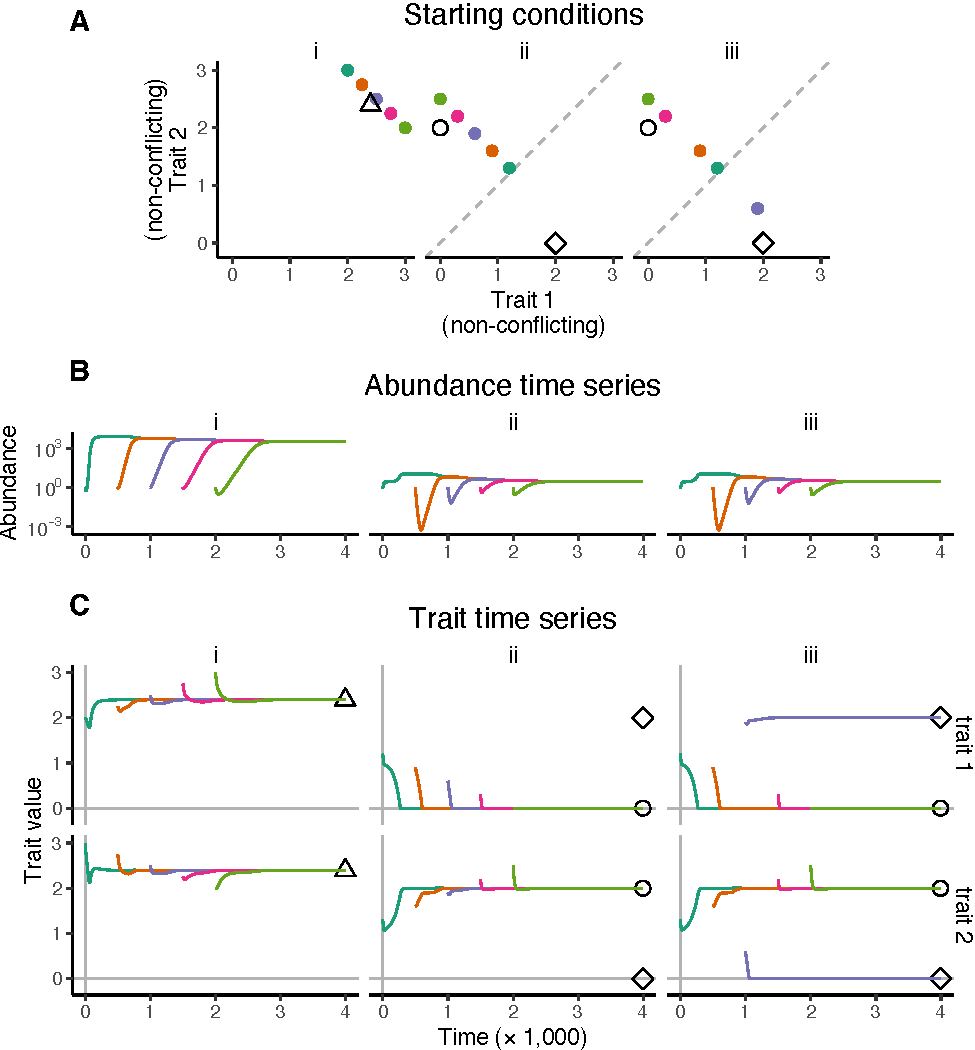
\includegraphics[width=\textwidth]{S1-cond_coexist_non-conflicting.pdf}
% \caption{Number of surviving species for 24 simulations of 2-trait 
%     communities
%     (A) after 50,000 generations for all permutations of the traits
%     being conflicting (``$-$'') or non-conflicting (``$+$''),
%     (B) after 50,000 generations for varying values of $d_2$ when 
%     $d_1$ is kept positive (i.e., trait 1 is kept non-conflicting), and
%     (C) through time with $d_2 = -10^{-2}$ and $d_2 = -10^{-4}$.
%     For all panels, $d_1 = 0.05$, $\eta = 0.6$, and species start with
%     random trait values ($\sim \text{N}(0,2)$ truncated $> 0$).
%     In (A), $d_2 = 0.1$.}
\caption{}
\label{fig:cond-coexist-non-conflicting}
\end{figure}


% \begin{figure}[ht!]
% \centering
% 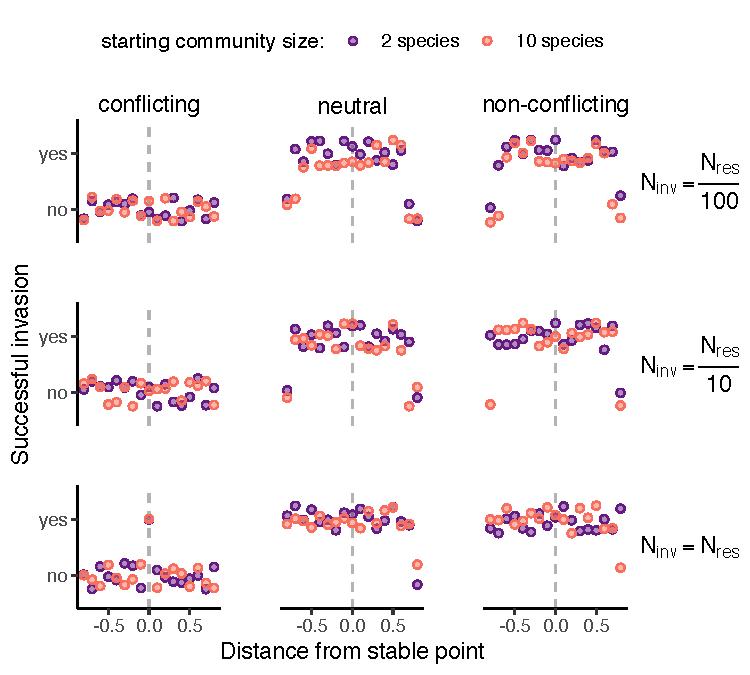
\includegraphics{S2-invasion.pdf}
% \caption{Invasion success for a 2-trait equilibrium community based on
%     the invader's starting distance from the equilibrium point in trait space.
%     Sub-panel columns indicate the type of evolution.
%     Sub-panels rows indicate the invaders' starting
%     abundances ($N_{eq}$) in relation to the residents'
%     abundances ($N_{res}$); all residents had the same
%     abundance.
%     Point color indicates the size of the resident community.
%     In these simulations, the resident community all had
%     trait values based on the analytical solutions for equilibria
%     in Appendix B.
%     The single invading species always had its first trait start
%     at the equilibrium value, but its second trait 
%     varied from
%     $-0.8$ to $0.8$ from the equilibrium value.
%     Simulations ran for 50,000 generations and assessed invasion 
%     success as the presence of the invader.
%     Here, $\eta = -0.6$, $d \in \{ -0.01, \; 0, \; 0.01 \}$.
% }
% \label{fig:invasion}
% \end{figure}

\begin{figure}[ht!]
\centering
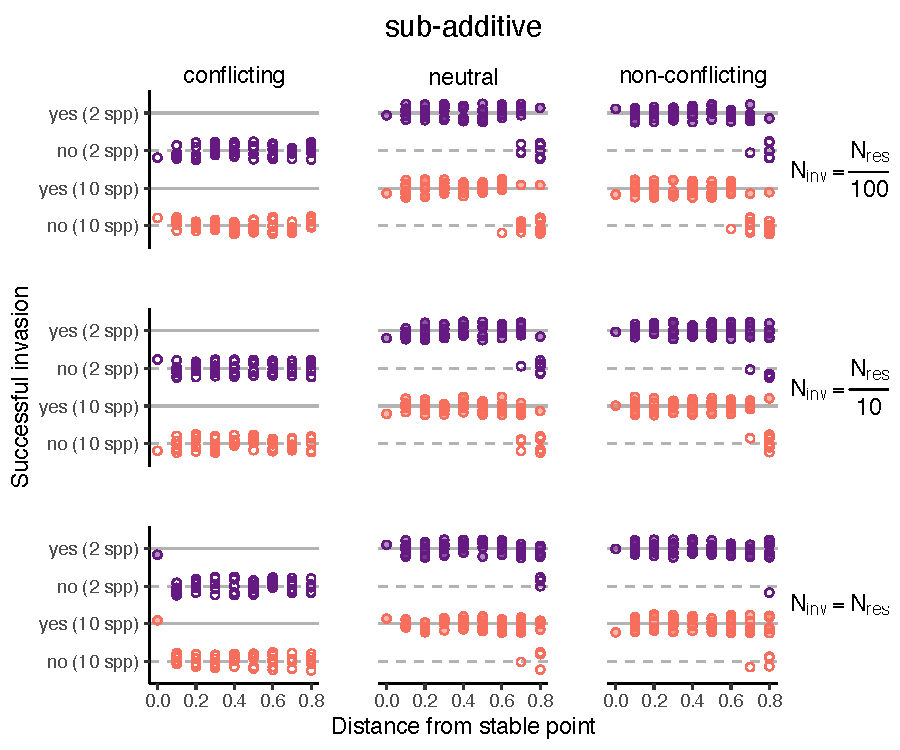
\includegraphics{S2-invasion_sub.pdf}
\caption{}
\label{fig:invasion-sub}
\end{figure}


\begin{figure}[ht!]
\centering
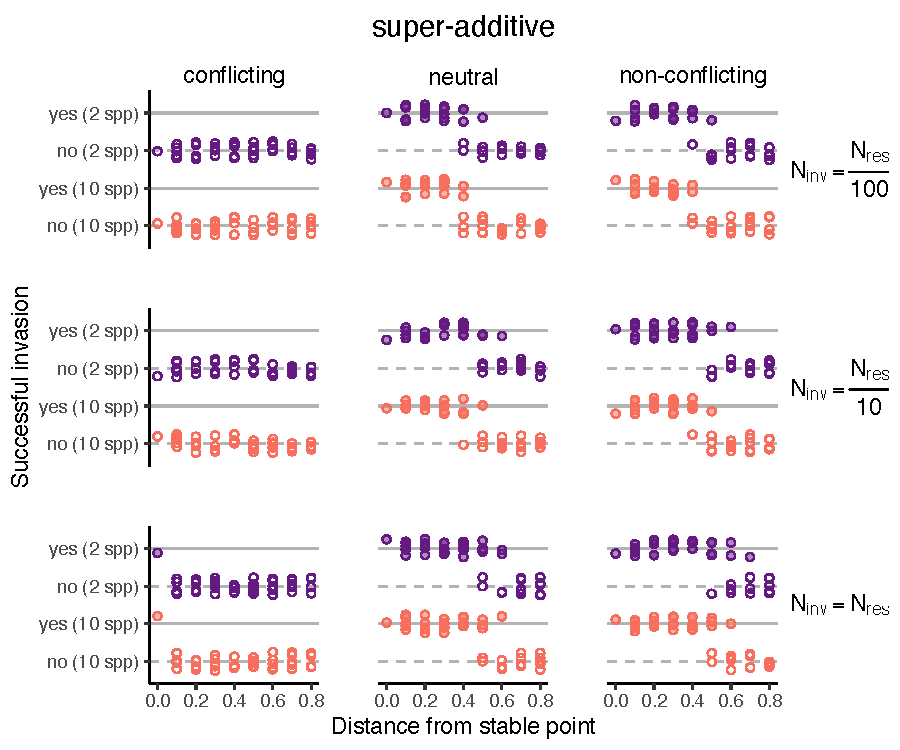
\includegraphics{S3-invasion_super.pdf}
\caption{}
\label{fig:invasion-super}
\end{figure}

